%!TEX root = ../../thesis.tex

\ac{QCD} is the theory of the strong interaction, describing coloured particles (quarks 
and gluons, collectively known as partons) \cite{Ellis:1996}. Two crucial features of 
\ac{QCD} are \textit{confinement} and \textit{asymptotic freedom}. Confinement refers to 
the observation that quarks and gluons are only found within colourless hadrons, and 
never as isolated states. Asymptotic freedom states that, within the hadron, the 
constituent partons are relatively free to move. Both concepts can be understood in terms 
of a running coupling constant.



\subsection{Renormalisation and the running coupling constant}
\label{sec:qcd:renormalisation}

When calculating observables within perturbative quantum field theory, ultraviolet (UV) 
divergences are often introduced by Feynman diagrams containing loops. Through careful 
consideration, these UV divergences can be absorbed into renormalised definitions of the 
coupling constant and particle masses. The idea is that the `bare' quantities contain 
compensating divergences, such that the physically measurable quantities are finite:
\begin{equation}
	g_{\text{physical}} = g_{\text{bare}} + \delta g
	\quad\quad\text{and}\quad\quad
	m_{\text{physical}} = m_{\text{bare}} + \delta m
\end{equation}
where $\delta g$ and $\delta m$ are the loop contributions. This procedure is known as 
\textit{renormalisation}.

It is necessary to introduce an unphysical \textit{renormalisation scale} \mur, above 
which loops are absorbed into renormalised quantities, and below which loops are 
calculated in perturbation theory. Clearly couplings and masses will depend upon \mur,
though physical observables must not -- however, truncation of the perturbative series 
will result in a residual \mur dependence. Usually \mur is chosen to be the energy 
scale $Q$ of the process under consideration, leading to the concept of a \textit{running 
coupling constant}.

The \ac{QCD} coupling constant \alphaS is shown in \Figure~\ref{fig:alpha_s}. At low 
scales (large distances), \alphaS is large and the theory is non-perturbative. 
Though not analytically proven\footnote{
	A mathematically rigorous proof of confinement is one of seven Millennium Prize 
	Problems of the Clay Mathematics Institute, with a bounty of \$1,000,000.
}, confinement has been verified in this regime by lattice \ac{QCD} \cite{Wilson:1974}. 
At high scales (small distances), \alphaS is small -- this is asymptotic freedom 
\cite{Gross:1973,Politzer:1973}. Note that \alphaEM in \acs{QED} exhibits an opposing 
trend, though remains perturbative at all accessible energies.
\begin{figure}
	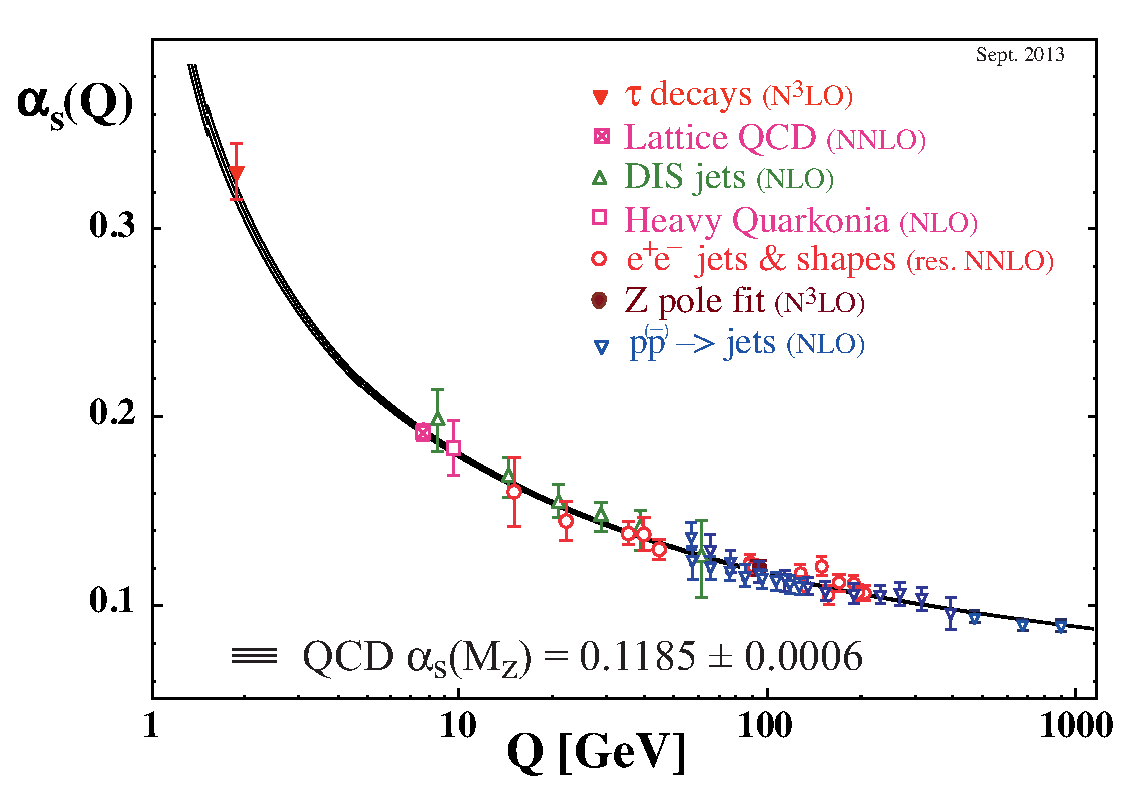
\includegraphics[width=\mediumfigwidth]{tex/tools/alpha_s}
	\caption{The running of the strong coupling constant \alphaS with energy scale $Q$ 
	\cite{PDG:2012}. Experimental measurements at various scales are also shown.}
	\label{fig:alpha_s}
\end{figure}



\subsection{Perturbative QCD}
\label{sec:qcd:pqcd}

Most interesting \acs{LHC} processes involve a large momentum transfer, where the partons 
are asymptotically free. Thus, parton-level cross sections may be calculated with Feynman 
diagrams as a perturbative series in \alphaS (which converges since $\alphaS \ll 1$)
\begin{equation}
	\hat{\sigma} = \sum\limits_{m=0}^{\infty} \alpha_{\text{S}}^{k+m} \hat{\sigma}^{(m)}
	\label{eq:qcd:partonic_xs}
\end{equation}
where the hat denotes a parton-level quantity, $k$ is the number of \ac{QCD} vertices at 
tree-level, and $\hat{\sigma}^{(m)}$ is the $m$th order contribution to the cross section.
A \textit{fixed order} calculation truncates the series after $n$ terms, with $n=0$ being 
a \ac{LO} calculation, $n=1$ being a \ac{NLO} calculation, and so on.

As mentioned in \Section~\ref{sec:qcd:renormalisation}, the cross section $\hat{\sigma}$ 
is independent of the renormalisation scale \mur
\begin{equation}
	\frac{\d{\hat{\sigma}}}{\d{\mur}} = 0 \,.
	\label{eq:qcd:xs_rge}
\end{equation}
However, real-life calculations always truncate the series after $n$ terms, leaving a 
residual \mur dependence. Inserting the truncated series into (\ref{eq:qcd:xs_rge}), 
it follows that
\begin{equation}
	\frac{\d{}}{\d{\mur}} \sum\limits_{m=0}^{n} \alpha_{\text{S}}^{k+m} \hat{\sigma}^{(m)}
	= \ofOrder{\alpha_{\text{S}}^{k+n+1}} \,.
\end{equation}
Thus, the residual \mur dependence can be exploited to probe the effect of missing 
higher order terms in the series, and estimate the associated uncertainty.

% In addition to the UV divergences handled by renormalisation, infrared (IR) divergences 
% arise from the soft and collinear emission of massless gluons. However, the 
% KLN theorem asserts that these cancel with IR divergences in corresponding loop 
% diagrams, and the cross section remains finite \cite{Kinoshita:1962,Lee:1964}.



\subsection{Resummation of large logarithms}
\label{sec:qcd:resum}

Fixed order calculations are useful only when the perturbative series is converging, as is
usual for an inclusive cross section. However, when considering exclusive observables, 
there are regions of phase space in which the missing higher order terms cannot be 
neglected. This often occurs when there is a large separation in the scales of a process.

For example, consider the emission of a gluon from an outgoing quark. The scale 
separation of the hard scatter $Q$ from the soft emission $Q_1$ introduces Sudakov double 
logarithmic contributions $\alpha_{\text{S}}^{k+m} L^{2m}$ to the perturbative series, 
where $L \sim \ln\parenths{Q_1 / Q}$. The (schematic) structure of the perturbative 
series becomes
\begin{equation}
	\hat{\sigma} \sim \alpha_{\text{S}}^k \braces{\alphaS \parenths{L^2 + L + 1}
	+ \alpha_{\text{S}}^2 \parenths{L^4 + L^3 + L^2 + L + 1} 
	+ \ofOrder{\alpha_{\text{S}}^3 L^6}} \,.
	\label{eq:qcd:resum}
\end{equation}
For soft or collinear emissions we have $\alphaS L^2 \approx 1$, and the logarithms can 
overcome the \alphaS suppression. Thus, the perturbative nature of the series is spoiled. 
In (\ref{eq:qcd:resum}), terms like $\alpha_{\text{S}}^{k+m} L^{2m}$ are called \acp{LL}, 
terms like $\alpha_{\text{S}}^{k+m} L^{2m-1}$ are called \acp{NLL}, and so on.

When sensitive to such large logarithms, they must be \textit{resummed} to all orders in 
\alphaS to produce an accurate result. This is usually achieved analytically, but in the 
case of the example soft and collinear emissions a \textit{parton shower} Monte Carlo 
program can be used. This probabilistically generates emissions as it evolves partons 
from the scale of the hard scatter down to a scale where non-perturbative effects of 
confinement dominate. This leads to fully-exclusive observables. A parton shower is 
necessary to produce hadron-level predictions (see \Section~\ref{sec:mc}). Technically 
they have \ac{LL} accuracy, though can include many \ac{NLL} terms such as 
energy-momentum conservation and colour coherence.



\subsection{Parton distribution functions}
\label{sec:qcd:pdf}

Since confinement binds partons into hadrons, it is these that are accelerated and 
collided at the \acs{LHC} (we consider protons in particular). Therefore, we need to 
calculate observables for proton-proton interactions rather than the parton-parton 
interactions discussed above. Fortunately, the \textit{factorisation theorem} states that 
the soft non-perturbative physics of the hadron can be treated independently of the hard 
scatter \cite{Collins:1982}. Thus, a proton-proton cross section can be formulated as a 
convolution of the partonic cross section with \acp{PDF} of the incoming protons. That is,
\begin{equation}
	\sigma\parenths{p_1, p_2} = 
	\sum\limits_{a, b} \! \int_0^1 \! \d{x_1} \d{x_2} \,
	f_a \parenths{x_1, \mu_{\text{F}}^2} f_b \parenths{x_2, \mu_{\text{F}}^2} \,
	\hat{\sigma}_{ab} \parenths{x_1 p_1, x_2 p_2, \alphaS\parenths{\mu_{\text{R}}^2}, 
	\frac{Q^2}{\mu_{\text{F}}^2}, \frac{Q^2}{\mu_{\text{R}}^2}} 
\end{equation}
where $f_a$ is the \ac{PDF} of parton type $a$ within the proton, $p_i$ is the momentum 
of proton $i$, and $x_i$ is the momentum fraction of parton $i$. A sum is performed over 
all possible parton types (six quark flavours and the gluon).

Echoing renormalisation, factorisation absorbs collinear divergences into universal 
\acp{PDF} which are not \textit{a priori} calculable and must be experimentally 
constrained. Again, an unphysical \textit{factorisation scale} \muf is introduced, 
below which emissions are absorbed into \acp{PDF}, and above which they are included in 
the hard scatter. As with \mur, truncating the perturbative series introduces a 
\muf dependence, which can be exploited to estimate the effect of the missing higher 
order terms. At \ac{LO}, $f_a \parenths{x, \muf}$ is simply the probability of finding a 
parton of type $a$ with momentum fraction $x$, when probing the proton at a scale \muf.
However, the interpretation at higher orders is more complex.

Crucially, the \ac{PDF} dependence upon \muf is described by the DGLAP equations 
\cite{Gribov:1972,Altarelli:1977,Dokshitser:1977}. This allows a $f_a \parenths{x}$ 
ansatz to be made at low scale and then experimentally validated at higher scales (\eg 
with deep inelastic scattering or collider jet data).
